\documentclass[a4paper,11pt]{article}

% Layout
\usepackage[a4paper, left=2.5cm, right=2cm, top=1cm, bottom=3cm]{geometry} % kleinere Ränder
\usepackage{parskip}

% Umlaute in der Datei erlauben, auf Deutsch umstellen
\usepackage{fontspec}
\usepackage{lmodern}
\usepackage[english, ngerman]{babel}

% Mathesymbole und Ähnliches
\usepackage{amsmath}
\usepackage{mathtools}
\usepackage{amssymb}
\usepackage{amsthm}
\usepackage{microtype}
\usepackage{stmaryrd}
\usepackage{MnSymbol}
\usepackage{bussproofs}		% Sequenzenkalkül
\usepackage{xcolor}

% Grafiken und PDFs einfügen
\usepackage{graphicx}
\usepackage{pdfpages}
\usepackage{float}

% PDF-Tools
\usepackage[hidelinks, unicode]{hyperref}

% Abbildungen
\usepackage{tikz}
\usetikzlibrary{arrows,calc,positioning}
\tikzset{ 
   state/.style={circle,fill,inner sep=2pt,label=below:#1\strut},
   arrow/.style={->, shorten <=3pt, shorten >=3pt, >=stealth',thick},
   knoten/.style={draw, circle, minimum size=8mm}} 
   
% Infoboxen 
\definecolor{orange}{RGB}{230,159,0}
\definecolor{darkgray}{RGB}{70,90,70}

\usepackage{tcolorbox}

\newenvironment{LP}[1]{%
\begin{minipage}{0.48\textwidth}
\begin{tcolorbox}[colback=orange!20!white, colframe=orange!80!black, title={\sffamily \textbf{#1}}]
}{
\end{tcolorbox}
\end{minipage}}

\newenvironment{alg}[1]{%
\begin{tcolorbox}[colback=red!15!white, colframe=red!85!black, title={\sffamily \textbf{#1}}]
}{
\end{tcolorbox}}

\newenvironment{info}[1]{%
\begin{tcolorbox}[colback=darkgray!15!white, colframe=darkgray!75!black, title={\sffamily \textbf{#1}}]
}{
\end{tcolorbox}}


% Reelle, Natürliche, Ganze, Rationale Zahlen
\newcommand{\R}{\ensuremath{\mathbb{R}}}
\newcommand{\N}{\ensuremath{\mathbb{N}}}
\newcommand{\Z}{\ensuremath{\mathbb{Z}}}
\newcommand{\Q}{\ensuremath{\mathbb{Q}}}

% Fraktur für Strukturen
\newcommand{\A}{\ensuremath{\mathfrak A}}
\newcommand{\B}{\ensuremath{\mathfrak B}}
\newcommand{\I}{\ensuremath{\mathfrak I}}

% Körper
\newcommand{\K}{\ensuremath{\mathcal{K}}}
%\newcommand{\G}{\ensuremath{\mathcal{G}}}

% Makros für logische Operatoren
\newcommand{\xor}{\ensuremath{\oplus}} % exklusives oder
\newcommand{\impl}{\ensuremath{\rightarrow}} % logische Implikation
\newcommand{\Lor}{\ensuremath{\bigvee}}
\newcommand{\Land}{\ensuremath{\bigwedge}}

% Meistens ist \varphi schöner als \phi, genauso bei \theta
\renewcommand{\phi}{\varphi}
\renewcommand{\theta}{\vartheta}

\newcommand*{\todo}{\textbf{\textcolor{red}{TODO}}}		% big, red, apparent TODO

% SEQUENZENKALKÜL
\usepackage{bussproofs}
\newcommand{\yields}{\ensuremath{\mathrel{\Rightarrow}}}

% Aufzählungen anpassen (alternativ: \arabic, \alph)
\renewcommand{\labelenumi}{(\roman{enumi})}

% BITTE NICHT ÄNDERN: interne Kommandos für die Informationen
\newcounter{sheet}
\newcommand{\printsheet}{\arabic{sheet}}


\newcommand{\printgroup}{?}
\newcommand{\group}[1]{%
\renewcommand{\printgroup}{#1}%
}

\newcommand{\printmembers}{}
\newcommand{\printmember}[3]{{#2} {#3} & {#1} \\}

\newtheorem{proposition}{Proposition}[sheet]

% Für Vektoren
\newcommand{\myvec}[1]{\ensuremath{\begin{pmatrix}#1\end{pmatrix}}}
\def\spvec#1{\left(\vcenter{\halign{\hfil$##$\hfil\cr \spvecA#1;;}}\right)}
\def\spvecA#1;{\if;#1;\else #1\cr \expandafter \spvecA \fi}

\newcommand{\pdfmembers}{}
\newcommand{\pdfmember}[3]{{#1} {#3}, {#2}; }

\newcommand{\member}[3]{%
\expandafter\renewcommand\expandafter\printmembers\expandafter{\printmembers\printmember{#1}{#2}{#3}}%
\expandafter\renewcommand\expandafter\pdfmembers\expandafter{\pdfmembers\pdfmember{#1}{#2}{#3}}%
}

\AtBeginDocument{\hypersetup{
    pdftitle = {Übungsblatt \printsheet},
    pdfauthor = {Abgabegruppe \printgroup: \pdfmembers},
    pdfsubject = {Concurrency Theory}
}}

% <-------- HIER alle Informationen eintragen ========================
\setcounter{sheet}{4} % Nummer des Blatts

% alle Gruppenmitglieder in der Form \member{Matrikelnummer}{Vorname}{Nachname}
\member{5481114}{Danje}{Petersen}
\member{5174511}{Marc}{Majohr}

\begin{document}

% Kopfzeile
{\raggedright
\begin{tabular}{l}
    Concurrency Theory \\
    SS 2024 \\
    \today{} \\
\end{tabular}}
\hfill
{\Large Übung 0\printsheet}
\hfill
\begin{tabular}{l l}
\printmembers
\end{tabular}
\hrule


% <-------- HIER beginnt die Lösung ========================

\section*{Aufgabe \printsheet.1}



\section*{Aufgabe \printsheet.2}



\section*{Aufgabe \printsheet.3}



\section*{Aufgabe \printsheet.4}
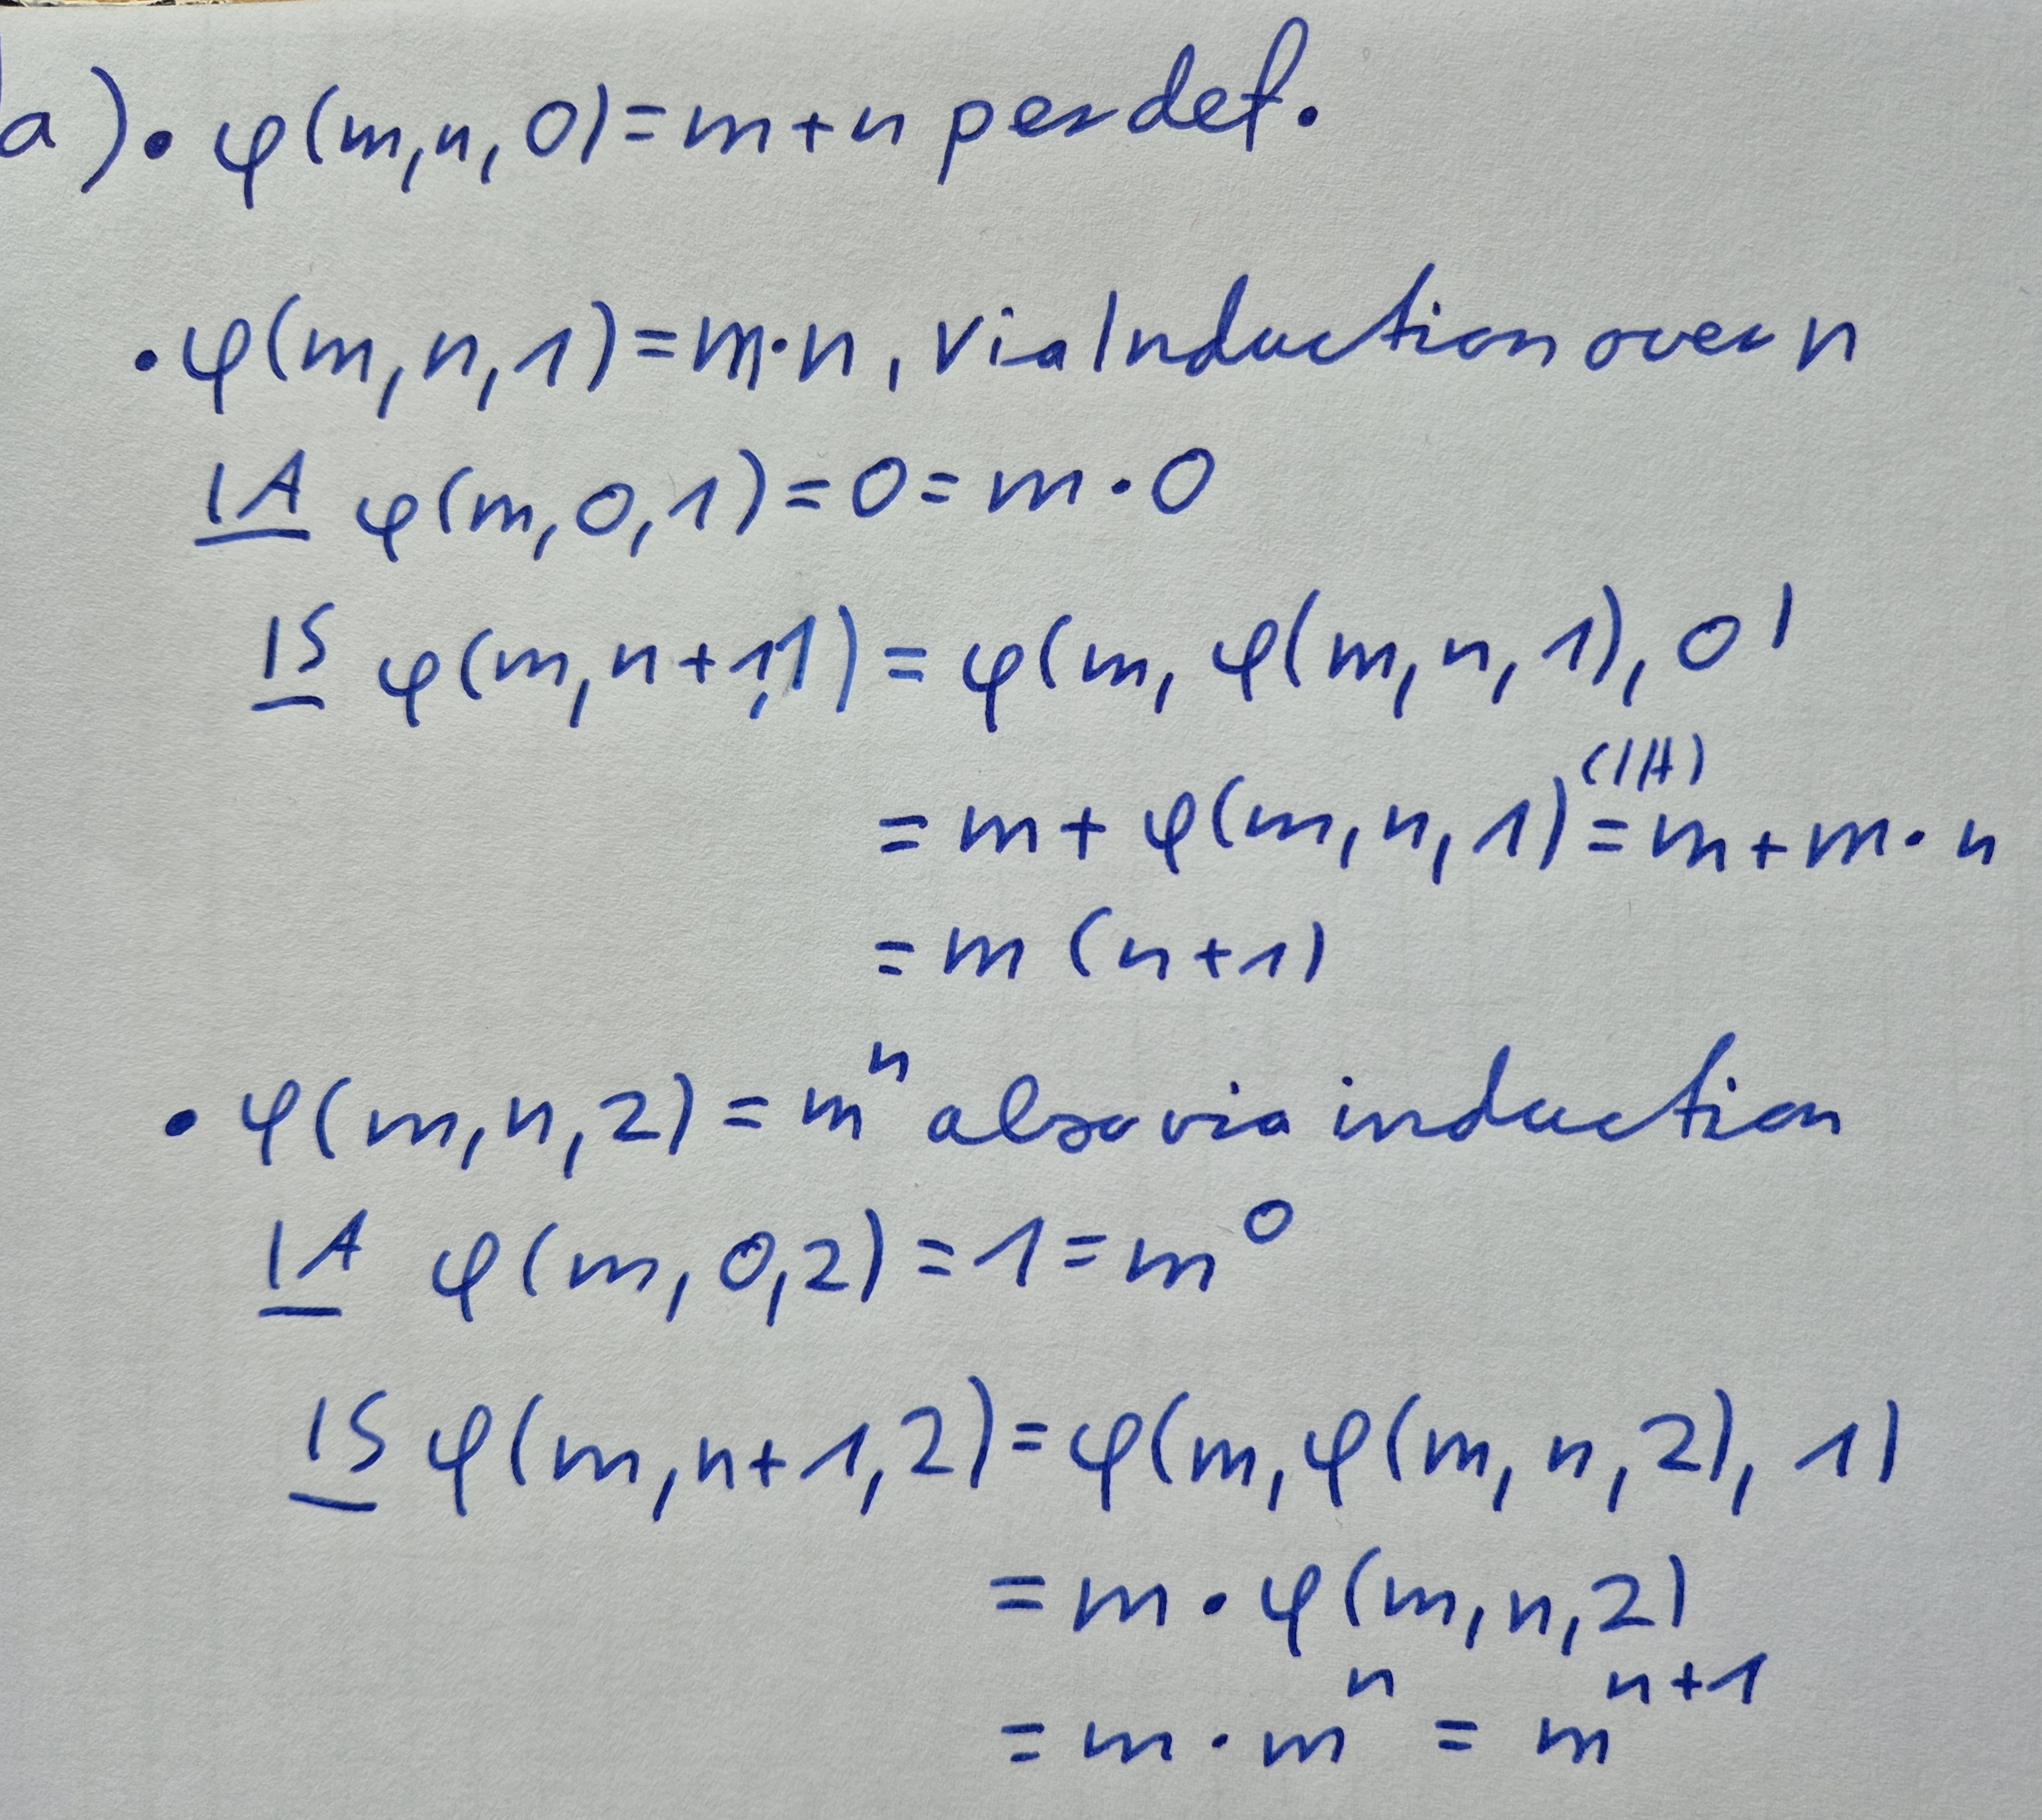
\includegraphics[scale=0.15]{4a}
\pagebreak
\subsection*{(b)}
\begin{align*}
A(2,3) &= A(1,A(2,2)) \\
&= A(1,A(1,A(2,1))) \\
&= A(1,A(1,A(1,A(2,0)))) \\
&= A(1,A(1,A(1,A(1,1)))) \\
&= A(1,A(1,A(1,A(0,A(1,0))))) \\
&= A(1,A(1,A(1,A(0,A(0,1))))) \\
&= A(1,A(1,A(1,A(0,2)))) \\
&= A(1,A(1,A(1,3))) \\
&= A(1,A(1,A(0,A(1,2)))) \\
&= A(1,A(1,A(0,A(0,A(1,1))))) \\
&= A(1,A(1,A(0,A(0,A(0,A(1,0)))))) \\
&= A(1,A(1,A(0,A(0,A(0,A(0,1)))))) \\
&= A(1,A(1,A(0,A(0,A(0,2))))) \\
&= A(1,A(1,A(0,A(0,3)))) \\
&= A(1,A(1,A(0,4) \\
&= A(1,A(1,5)) \\
&= A(1,A(0,A(1,4))) \\
&= A(1,A(0,A(0,A(1,3)))) \\
&= A(1,A(0,A(0,A(0,A(1,2))))) \\
&= A(1,A(0,A(0,A(0,A(0,A(1,1)))))) \\
&= A(1,A(0,A(0,A(0,A(0,A(0,A(1,0))))))) \\
&= A(1,A(0,A(0,A(0,A(0,A(0,A(0,1))))))) \\
&= A(1,A(0,A(0,A(0,A(0,A(0,2)))))) \\
&= A(1,A(0,A(0,A(0,A(0,3))))) \\
&= A(1,A(0,A(0,A(0,4)))) \\
&= A(1,A(0,A(0,5))) \\
&= A(1,A(0,6)) \\
&= A(1,7) \\
&= A(0,A(1,6)) \\
&= A(0,A(0,A(1,5))) \\
&= A(0,A(0,A(0,A(1,4)))) \\
&= A(0,A(0,A(0,A(0,A(1,3))))) \\
&= A(0,A(0,A(0,A(0,A(0,A(1,2)))))) \\
&= A(0,A(0,A(0,A(0,A(0,A(0,A(1,1))))))) \\
&= A(0,A(0,A(0,A(0,A(0,A(0,A(0,A(1,0)))))))) \\
&= A(0,A(0,A(0,A(0,A(0,A(0,A(0,A(0,1)))))))) \\
&= A(0,A(0,A(0,A(0,A(0,A(0,A(0,2))))))) \\
&= A(0,A(0,A(0,A(0,A(0,A(0,3)))))) \\
&= A(0,A(0,A(0,A(0,A(0,4))))) \\
&= A(0,A(0,A(0,A(0,5)))) \\
&= A(0,A(0,A(0,6))) \\
&= A(0,A(0,7)) \\
&= A(0,8) \\
&= 9
\end{align*}




\end{document}
